\documentclass[11pt]{article}
\usepackage{amsmath}
\newcommand{\numpy}{{\tt numpy}}    % tt font for numpy
\usepackage{graphicx}

\topmargin -.5in
\textheight 9in
\oddsidemargin -.25in
\evensidemargin -.25in
\textwidth 7in

\begin{document}

% ========== Edit your name here
\author{Yida Liu}
\title{MSOR 411: Homework 1: Due by 4:30pm Monday, September 09, 2019}
\maketitle

\medskip

% ========== Begin answering questions here
\begin{enumerate}



\item
\textbf{Answer to question 1 }\par

For the following problems, I used the following guideline in the trial-and-error approach.

\begin{itemize}
    \item Set all the variable to their minimum requirement.
    \item Select the most constrained variable and increase it until it cannot be increased any more (i.e. one or more constraints at the limits).
    \item Try increase other variables that does not affect the constraints that are on the limits. 
\end{itemize}

The following section displays the EXCEL screeshots for the models.
\begin{enumerate}

\item Blubbermaid\par

\begin{center}
            \includegraphics[width=\linewidth]{{bubblermaid_screenshot}}
\end{center}

\item MakeOrBuy

\begin{center}
    
        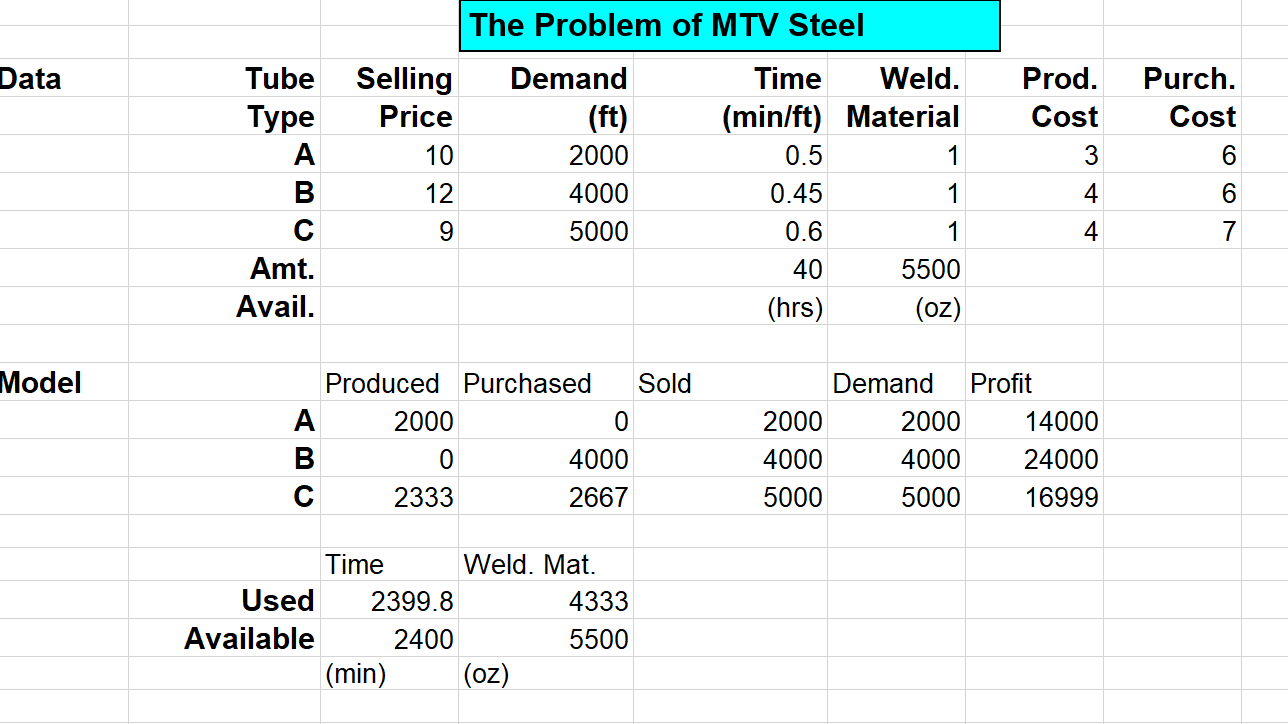
\includegraphics[width=\linewidth]{makeorbuy_screenshot.png}
\end{center}


\item Energy problem of Lilliput

\begin{center}
            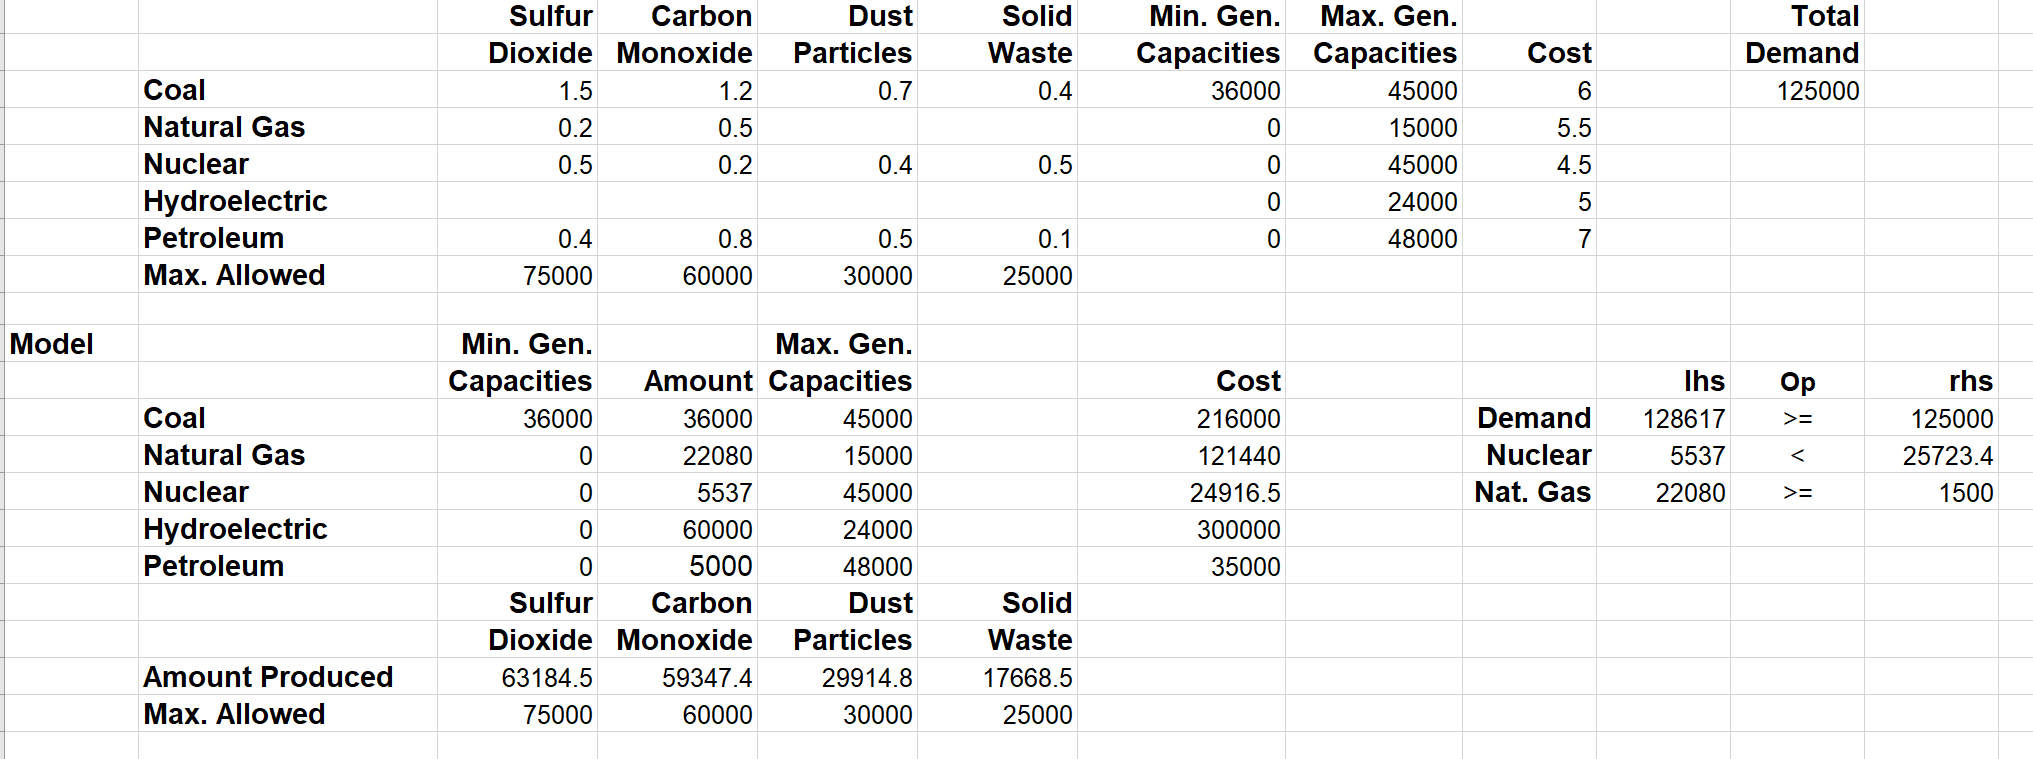
\includegraphics[width=\linewidth]{energy_screenshot.png}
\end{center}
\end{enumerate}

\item \textbf{ Answer to question 2}

\renewcommand{\labelenumii}{{\arabic{enumii}}}
\begin{enumerate}
    \item Unsure where to stop\par
    When increasing the variables, it is hard to tell when to stop. The only solution is to keep trying until the specific combination of variable satisfies all constraints.
    \item Does not scale \par
    The trial-and-error approach might only work for small problems that could come with answers with only small number of iterations. However, for large problems, even slightly larger, it is hard for human to manually do the computation.
    \item Hard to "Debug" model\par
    If a false / erroneous model was established at the beginning, it is hard to tell until some obvious errors are visible for humans.
\end{enumerate}

\item \textbf{ Answer to question 3: Fresh Diary Farms} \par

For this question, we follow the procedure introduced in class to build the model for the Fresh Diary Farms problem.

\renewcommand{\labelenumii}{{\arabic{enumii}}}
\begin{enumerate}
    \item Identify the variables\par
    The values that constitutes the solution to the Fresh Diary Farms problem is the production plan, which are the production quantity low-fat milk, butter, and cheese. We denote these three variables as:
    \begin{itemize}
        \item $L$: the total quantity of low-fat milk produced daily as gal
        \item $B$: the total quantity of butter produced daily as in lb
        \item $C$: the total quantity of cheese produced daily as in lb
    \end{itemize}
    \item Identify the objective function\par
    The goal for the problem is to maximize the profits of the farm with an production plan, which were discussed in the first step. The profits consists of the sale of low-fat milk, butter, and cheese produced, respectively. At the same time, the unit profit of each product is provided by the problem. Therefore, we could formulate the following equation as the objective function of the Diary Farm Problem:
    $$
    \max_{L, B, C} 0.22L + 0.38B + 0.72C
    $$
    \item Identify the constraints\par
    The constraints for this problem can be categorized into 3 different types: resource constraints, demand constraints, and logical constraints. We discuss these types accordingly.
    
    \begin{itemize}
        \item Resource constraints\par
        \begin{itemize}
            \item Machine Utilization\par
            Fresh Diary Farms has two different machines that both could process raw milk into the three products: low-fat milk, butter, and cheese. However, the processing speed differs by products and machines. There is an upper limit for the machine utilization of 8 hours (or 480 minutes) per day. Therefore, the production plan must cope with the limitations. Moreover, we introduce a subscript $i$ for the aforementioned symbols for each of the products to denote the machine-independence for each products:
            
            \begin{align*}
                L &= \sum_i L_i \\
                B &= \sum_i B_i \\
                C &= \sum_i C_i
            \end{align*}
            
            where $i\in [1..2]$. Hence, we denote the machine utilization constraint as:
            \begin{align*}
                0.2 L_1 + 0.5 B_1 + 1.5 C_1 & \leq 480 \\
                0.3 L_2 + 0.7 B_2 + 1.2 C_2 & \leq 480
            \end{align*}
        \end{itemize}
        \item Demand constraints\par
        \begin{itemize}
            \item Minimum Required\par
            There is a lower limit for the amounts in the production plan, which can be expressed as
            \begin{align*}
                L = \sum_i L_i & \geq 300 \\
                B = \sum_i B_i & \geq 200 \\
                C = \sum_i C_i & \geq 100
            \end{align*}
        \end{itemize}
        
        \item Logical Constraints\par
        $$
        \text{All Variables} \geq 0
        $$
    \end{itemize}
    
    \item Is this a linear programming problem?\par
    With the above three steps, we could formulate the optimization model for the Diary Farm Problem as follows:
    \begin{align*}
        &\max_{L_i, B_i, C_i, \forall i \in [1..2]}&&0.22\sum_i L_i + 0.38\sum_i B_i + 0.72\sum_i C_i  \\
        &s.t.&&0.2 L_1 +        0.5 B_1 +       1.5 C_1  \leq 480 \\
        &    && 0.3 L_2 +     0.7 B_2  +       1.2 C_2  \leq 480 \\
        &    && \sum_i L_i  \geq 300 \\
        &   && \sum_i B_i  \geq 200 \\
        &   && \sum_i C_i \geq 100 \\
        &   && \forall i \in [1..2], L_i, B_i, C_i \geq 0
    \end{align*}
    
    The above model is a linear model, since the objective function, all decision variables and all constraints are all linear
\end{enumerate}

\item \textbf{Answer to question 4: Leather Company} \par

\renewcommand{\labelenumii}{{\alph{enumii}}}
\begin{enumerate}
    \item Identify the variables \par
    In the Leather Company problem, the manager would like to decide a production plan for each of the products, which are baseball gloves, footballs and leather straps, respectively. Therefore, the decision variable in the production plan would be the quantity of each type of the products. Here, we denote use the following symbols to denote the production plan:
    \begin{itemize}
        \item $G$: the total number of pairs of baseball gloves produced weekly.
        \item $F$: the total number of footballs produced weekly.
        \item $S$: the total number of leather straps produced weekly.
    \end{itemize}
    \item Identify additional data \par
    It is easy to notice that the data provide by the problem body is not sufficient for us to build a mathematical model. Additional data is needed for us to formulate the model for the Leather Company problem. We present the following list of symbols to denote the additional data needed and we use the subscript to denote the attribute for each specific variables. 
    \begin{itemize}
        \item $P$: the unit profit for selling one unit of product in dollar. \par
        \{$P_G, P_F, P_S$\}
        \item $\mathit{CL}$: the leather consumption for producing one unit of product in square meters.\par
        \{$\mathit{CL}_G, \mathit{CL}_F, \mathit{CL}_S$\}
        \item $\mathit{TM}$: the machine time usage for producing one unit of product in minutes. \par
        \{$\mathit{TM}_G, \mathit{TM}_F, \mathit{TM}_S$\}
    \end{itemize}
    
    \item Formulate a model.
    \renewcommand{\labelenumiii}{{\arabic{enumiii}}}
    \begin{enumerate}
        \item Identify objective function\par
        The goal for the problem is maximize the profit gained from selling the product, which could be written as
        $$
        max_{G, F, S} P_GG + P_FF+ P_SS
        $$
        \item Identify constraints \par
        \begin{itemize}
            \item Resource constraints\par
            \begin{itemize}
                \item Material Availability \par
                The total number of leather availability is limited to 1000 square meters.
                $$
                \mathit{CL}_GG+ \mathit{CL}_FF+ \mathit{CL}_SS \leq 1000
                $$
                \item Machine Utilization\par
                The machine utilization could not exceed 40 hours (2400 minutes) every week.
                $$
                \mathit{TM}_GG + \mathit{TM}_FF+\mathit{TM}_SS \leq 2400
                $$
            \end{itemize}
            \item Demand constraints\par
            Unless otherwise specified, there is no demand constraints under the problem setting.
            \item Logical constraints\par
            All variables must be greater than zero.
            $$
            \text{All variable} \geq 0
            $$
        \end{itemize}
        \item Is the model a linear model?
        Gather all the information above, we formulate the mathematical model for this problem as follows:
        \begin{align*}
            & \max_{G, F, S} & & P_GG + P_FF+ P_SS  \\
            & s.t. && \mathit{CL}_GG+ \mathit{CL}_FF+ \mathit{CL}_SS \leq 1000 \\
            &&& \mathit{TM}_GG + \mathit{TM}_FF+\mathit{TM}_SS  \leq 2400 \\
            &&& G, F, S \geq 0
        \end{align*}
        
        This model is not a linear model because the decision variables ($G,F,S$) is not continuous, as in the sense that the Lether Company cannot sell 0.5 football. 
    \end{enumerate}
\end{enumerate}

\item \textbf{Answer to question 5: Florida Citrus Inc.} \par

Following the standardized procedure for obtaining a mathematics model, we build a model for the Florida Citrus Inc. to maximize the profit.

\renewcommand{\labelenumii}{{\arabic{enumii}}}
\begin{enumerate}
    \item Identify the variables\par
    The central problem for the Florida Citrus Inc. is to maximize the profit for selling orange and grapefruit concentrate. Their profit solely depends on the sales of these two concentrate. Thus, we identify the following decision variable:
    \begin{itemize}
        \item $CT$: the volume of the concentrate produced by Florida Citrus Inc. in gallon. \{$CT_O$: volume of orange concentrate produced, $CT_G$ : volume of grapefruit concentrate produced\}
    \end{itemize}
    \item Identify the objective function\par
    The sales of concentrates is the only source of the profit and at the same time, the raw materials, grapefruit and orange juice, incur costs to produce the final product. Following the notation of the problem, we obtain the following objective function:
    $$
    \max_{\mathit{CT_O}, \mathit{CT_G}} 6\mathit{CT_O} + 8\mathit{CT_G} - 1.5\mathit{OJ} - 2\mathit{GJ}
    $$
    Before we proceed to identify the constraints, we also identify the following equality constraints for juice and concentrates:
    \begin{align*}
        0.7 \mathit{OJ} &= \mathit{CT_O} \\
        0.75 \mathit{GJ} &= \mathit{CT_G}
    \end{align*}
    Thus, the objective function further simplifies to
    \begin{align*}
        \max_{\mathit{OJ}, \mathit{GJ}} 2.7\mathit{OJ} + 4\mathit{GJ}
    \end{align*}
    \item Identify the constraints\par
    \begin{itemize}
        \item Resource constraints\par
        \begin{itemize}
            \item Machine Utilization\par
            The distillation machine has a limited utilization of 80 hours per week. The production plan must not over-utilize the machine to avoid potential problems that might cause. 
            $$
            \frac{1}{25} \mathit{OJ} + \frac{1}{20} \mathit{GJ} \leq 80 
            $$
        \end{itemize}
        \item Demand constraints\par
        \begin{itemize}
            \item Storage capacity\par
            The storage capacity for each type of concentrate are limited to 1000 gallons.Therefore, the storage capacity constraints could be written as:
            \begin{align*}
                  \mathit{CT_O} = 0.7 \mathit{OJ} & \leq 1000  \\
                 \mathit{CT_G} = 0.75 \mathit{GJ} & \leq 1000 
            \end{align*}
        \end{itemize}
        
        \item Logical constraints\par
            All variables must be greater than zero.
            $$
            \text{All variable} \geq 0
            $$    
    \end{itemize}
    \item Formulate the model \par
    Based on all the information we obtained above, we could formulate a mathematical model for the Florida Citrus Inc. to maximize their profit. 
    \begin{align*}
        & \max_{\mathit{OJ}, \mathit{GJ}} & & 2.7\mathit{OJ} + 4\mathit{GJ} \\
        & s.t. & & \frac{1}{25} \mathit{OJ} + \frac{1}{20} \mathit{GJ} \leq 80 \\
        &&&  0.7\mathit{OJ} \leq 1000  \\
        &&& 0.75 \mathit{GJ}  \leq 1000 \\
        &&& \mathit{OJ}, \mathit{GJ} \geq 0
    \end{align*}
\end{enumerate}

\end{enumerate}

\end{document}
\grid
\grid